\documentclass[a4paper, 11pt, twocolumn]{article}

\usepackage[utf8]{inputenc}

\usepackage[T1]{fontenc}

\usepackage[english]{babel}

\usepackage{graphicx}

 \usepackage{floatrow}

\usepackage[margin = 1in]{geometry}

\usepackage{float}

\usepackage[hidelinks]{hyperref}


\usepackage{url}

\usepackage{natbib}

%\usepackage[
%backend=biber,
%sorting=none
%]{biblatex}
\bibliographystyle{abbrvnat}
\setcitestyle{authoryear,open={(},close={)}}

\usepackage[most]{tcolorbox}

\usepackage{csquotes}

\usepackage{fancyhdr}


\usepackage{lipsum}

%\addbibresource{references.bib}

\title{\Large Internship report \\
\huge Alternative PCA algorithms analysis with missing values}


\author{Léopold Guyot}

\date{\today}

\begin{document}

\pagestyle{fancy}
\setlength{\headheight}{25.0117pt}
\fancyhead{}\fancyfoot{}
\fancyhead[L]{
\includegraphics[width = 0.2\textwidth]{UCLouvain_Logo_Pos_CMJN.pdf}}
\fancyhead[R]{Alternative PCA algorithms analysis with missing values}
\fancyfoot[R]{\thepage}

\onecolumn
\maketitle

\begin{tcolorbox}[breakable,colback=white,colframe=black,width=\dimexpr\textwidth+12mm\relax,enlarge left by=-6mm]

\section*{Abstract}
Principal Component Analysis (PCA) is commonly used in single-cell proteomics (SCP), but most used PCA algorithm don't support missing values, therefore the data require imputation methods that can introduce biases. This report explores PCA methods that work on missing values, specifically NIPALS and PPCA, in SCP. Real SCP data is used to evaluate the impact of missing values on cell arrangement in the PCA space and assess downstream analysis. Results show that NIPALS and PPCA yield comparable PCA results to SVD. Changes in local cell arrangement are observed with increasing missing value rates, but overall patterns remain similar. NIPALS should become the preferred method to perform PCA on SCP data set, this way avoiding imputation drawbacks.

\end{tcolorbox}

\begin{figure}[H]
          \begin{minipage}{.5\textwidth}
                \centering
                
\includegraphics[width = \linewidth]{UCLouvain_Logo_Pos_CMJN.pdf}
          \end{minipage}
           \begin{minipage}{.5\textwidth}
           \centering
                
\includegraphics[width = 0.7\linewidth]{institut.png}
          \end{minipage}
\end{figure}

\twocolumn
\section{Introduction}

Principal Component Analysis (PCA) is a widely used dimension reduction method in the omics field, including single-cell proteomics (SCP). However, traditional PCA methods like singular value decomposition (SVD) cannot handle missing values, which can be a significant challenge in data sets with high percentages of missing values, such as SCP data where it can reach up to 90\% missing values.

Imputation, the process of predicting missing values, is often necessary before applying PCA or downstream analysis. However, imputation methods have several limitations \citep{vanderaa_revisiting_2023}. First, it can introduce biases. Biased estimates can arise if an unsuitable imputation model is used. Second, imputation may also reduce biological heterogeneity as imputed values are based on combined observed values, masking the true variability. Finally, imputation can obscure inestimable contrasts that may hold important biological information.
Given these drawbacks, careful consideration of imputation methods is crucial in SCP data analysis.

There are some alternative methods that could replace the imputation step. In proteomic, some models are used to take missing values into account, they contain several components one of which is present to modelling the missing rates \citep{goeminne_msqrob_2020, obrien_effects_2018}. It could be a efficient solution but these models are limited in term of downstream analyses and are not suitable for SCP. In the single cell RNA Sequencing field, some models have been developed that use dimension reduction while accounting for missing values \citep{risso_general_2018}. But these models are not developed for SCP. An implementation of this kind model in SCP could be a compelling solution. An other solution would be to run a dimension reduction on the data with missing values, here the missing values are considered missing at random. This can be achieved with an alternatives PCA method, for exemple the Non-linear Iterative Partial Least Squares or NIPALS. It is an algorithm that computes iteratively each PCs, it can be used in presence of missing values \citep{preda_nipals_2010}. With this kind of PCA, the analysis can start with an incomplete data set with missing values, and obtain a dimension reduction with scores containing only complete values, therefore allowing for visualisation or downstream analyses. In this report NIPALS and an other NAs-compatible PCA, PPCA (probabilistic pca \citep{tipping_probabilistic_1999}) will be tested with real single cell data. The first goal is to estimate the impact of the missing values on the spatial location of cells in the PCs space. In others words the goal is to understand if the PCA results with no imputation produces results similar to the PCA on complete data. Then the dimension reduction efficiency will be tested by using a downstream analysis. This analysis will be the measure of the accuracy of the clustering obtained with PCA made with different rates of missing values. And then, the different time performance implementations of the PCA algorithms will be compared. 

\section{Methods}

The analysis presented in this report utilized R programming language \citep{Rlang}. The data set used in the analysis was obtained from Leduc (2022) \citep{Leduc2022}, who employed the improved SCoPE2 protocol with the CellenONE liquid handling system. The data set includes quantitative information on melanoma cells and monocytes at the PSM, peptide, and protein levels. Specifically, the "proteins\_norm2" assay, contained within a SingleCellExperiment object \citep{SingleCellExperiment}, was utilised. This assay comprises quantitative protein data for 2844 proteins and 1543 single cells. The data was retrieved using the scpdata package \citep{scpdata}.
Three different analyses were conducted using the proteins\_norm2 assay. In each analysis, batch correction was performed using the "Set" variable, that represents the acquisition groups. Two PCA algorithms, nipals and ppca, from the pcaMethods package \citep{pcaMethods}, were employed to compare their performance. Additionally, the svd method from the same package was used to perform a classical PCA, like in the widely-used prcomp function from the stats package \citep{Rlang}.
In the first analysis, a subset of the data set was created, consisting of 445 proteins and 152 cells, without any missing values. Subsequently, 19 additional subsets were generated, introducing missing values with rates ranging from 0\% to 95\%. Missing values were randomly generated within each subset. Dimension reduction using 15 principal components (PCs) was performed with nipals and ppca. The Euclidean distance and Pearson correlation between pairs of points in the PC space were computed using functions from the stats package \citep{Rlang}. Differences in correlation and distance, compared to the complete subset (0\% missing values), were calculated for each missing value rate.
In the second analysis, the entire proteins data set was used. The first step involved imputing the missing values using the impute function from the scp package \citep{scp}. 19 sets were generated with varying missing value rates. Only the imputed values were transformed in NAs. When all of them were transformed the generation started to be random (>65\% of NAs). To estimate the variability caused by the random generation, each missing value rate were replicated ten times. PCA was performed on each set using nipals, ppca, and svd (only for the set without missing values). The resulting PCs were subjected to the kmeans unsupervised clustering algorithm from the stats package \citep{Rlang}. The accuracy of clustering results, indicating the rate of correctly classified cells, was computed by comparing the clusters with the real groups of cells.
The last analysis focused on measuring the computational time taken by each algorithm. Nipals, ppca, and svd (with or without considering imputation in the time measured) were applied to subsets of various sizes, ranging from 300 proteins by 200 cells ($n = 6 \times 10^4$) to the full data set ($n = 4.2 \times 10^6$). This was done using 2, 10, and 25 PCs. To obtain results of the average time taken by the algorithms, each parameter combination was replicated ten times. Time measurements were conducted using the microbenchmark package \citep{microbenchmark}. 

For some of the analysis, statistic tests were used. To test the mean differences between groups, a simple linear model was employed. To test the difference in variance between groups, a Levene Test \citep{car} was employed.

Each scripts and markdowns used for this report can be found at \url{https://github.com/leopoldguyot/Internship_report_july_2023}.





\section{Results}

\subsection{Impact of the missing values on the spatial arrangement of cells in the PCs space}

\subsubsection*{NIPALS}

The PCAs obtained with NIPALS seem to have decreasing values of explained variance by PCs as the NA rate increase (Fig. \ref{corr_dist_nipals}B). This means that as the occurrences of missing values increase, less of the variability of the data can be caught within a PC. The scale of each PCA seems to decrease as the missing value rate raises. On the PCA plot with 0\% NA, the scale goes from -10 to 10, as for the 90\% PCA plot, the scale goes from -2 to 2. This scale variability explains why the distance between each pair of points is decreasing (linear model : pvalue <2e-16) with the increase of the missing value rate (Fig. \ref{corr_dist_nipals}A). Therefore the PCA scores were normalised, so that each PC has the same weight. The distance obtained with these normalised scores from now on will be named the normalised distance. With this transformation, the metric seems stable. A similar measure was made using the correlation. With this metric only the relation (increase or decrease) between each pair of points, therefore it is not impacted by the scale variability of the PCs. Correlation is stable similarly to the normalised distance. The stability of these two metrics indicates that the overall pattern of each PCA stays similar with the increase of NAs. 

\begin{figure*}[!ht]
    \textbf{NIPALS PCA distance and correlation analysis}
    \centering
    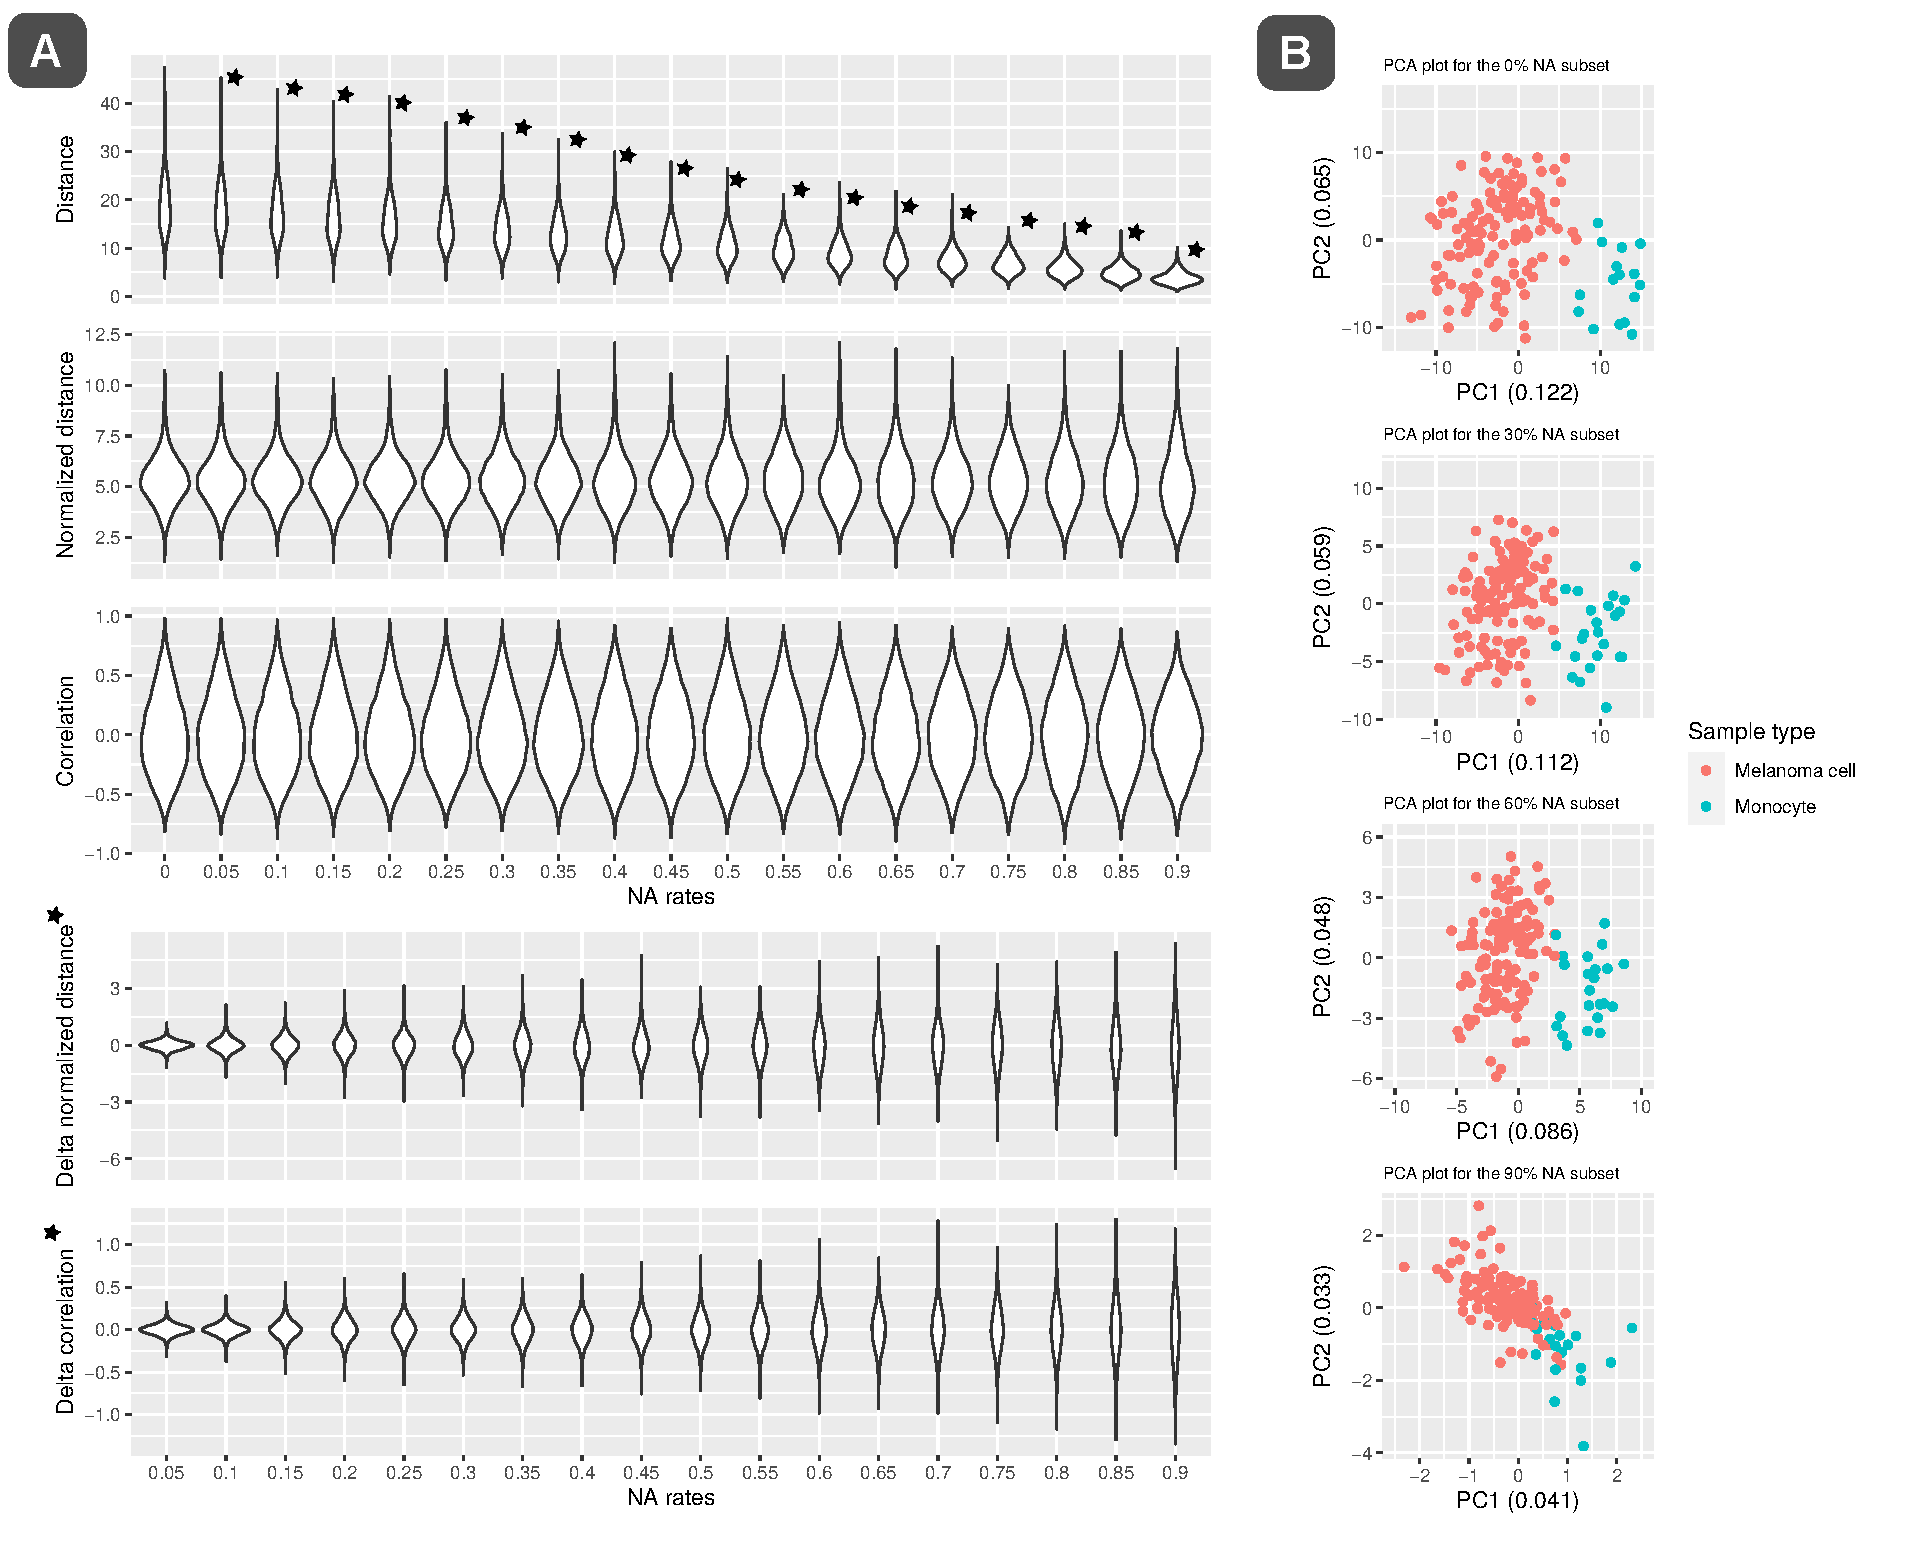
\includegraphics[width = \linewidth]{nipals_merged.pdf}
    \caption{\small (A) Five graphs representing each metric for each missing value rate in the data set. \scriptsize The metrics were computed on the PCA made with nipals from pcaMethods. Be aware that the 3 first graphs start with the 0\% missing value data set but the two last graphs start with 5\% of missing values. Asterisks into graph indicate the pvalue of the linear model test between the result and the reference (first group in the graph) . When asterisks are outside a graph they indicate that the total pvalue is inferior to 0.05
    \small (B) Four PCA plot for 0\%, 30\%, 60\% and 90\% missing value rate. \scriptsize Numbers between parentheses on axis title stand for the proportion of variability that is explained by the PC. Blue points represent Monocyte cells, red points represent Melanoma cells.
    }
    \label{corr_dist_nipals}
\end{figure*}

To identify the changes within the pattern, the difference between the normalised distance from the PCA obtained with the 0\% missing value data set and the normalised distance from the PCA of each of the other percentage of NA was computed. Same was done using the correlation. This difference from now on will be named delta. Both delta normalised distance and delta correlation show an increase (Levene Test : pvalue <2e-16) in the values of the difference (positively or negatively). This indicates that even if the overall pattern of the cells is similar for all NA rates, the localisation within the pattern seems to change. This change becomes bigger as the missing value rate increases. This means that the insertion of missing values has an effect, but this effect does not affect the overall pattern of each PCA. 

A closer look to some PCA plots (Fig. \ref{corr_dist_nipals} B), shows graphically that the two clusters seem to overlap more.



\subsubsection*{PPCA}

The PCAs obtained with PPCA get increased values of explained variance by PCs as the NA rate increases (Fig. \ref{corr_dist_ppca}B). This is the opposite to the results from NIPALS. Also, the scale of each PCA seems to increase as the missing value rate raises. On the PCA plot with 0\% NA, the scale go from -20 to 10,  for the 90\% PCA plot the scale go from -20 to 20. This scale variability explain why the distance between each pair of points is decreasing (linear model : pvalue <2e-16) with the increase of the missing value rate (Fig. \ref{corr_dist_ppca}A). The fact that NIPALS and PPCA show opposite results has not yet found an explanation. An hypothesis could be that PPCA use an imputation during is computation, this could increase the variation in the data, therefore increasing the explained variance for each PC. The distance for the 90\% missing rate PCA appears to be a surprising, this may be caused by the implementation of the probabilistic pca. In line with NIPALS, distance was computed on normalised scores. With this transformation, the metric seems stable. Correlation is stable too. The stability of these two metrics indicates that the overall pattern of each PCA stays similar with the increase of NAs, this is the same as for NIPALS. 

\begin{figure*}[!ht]
   \textbf{PPCA distance and correlation analysis}
    \centering
    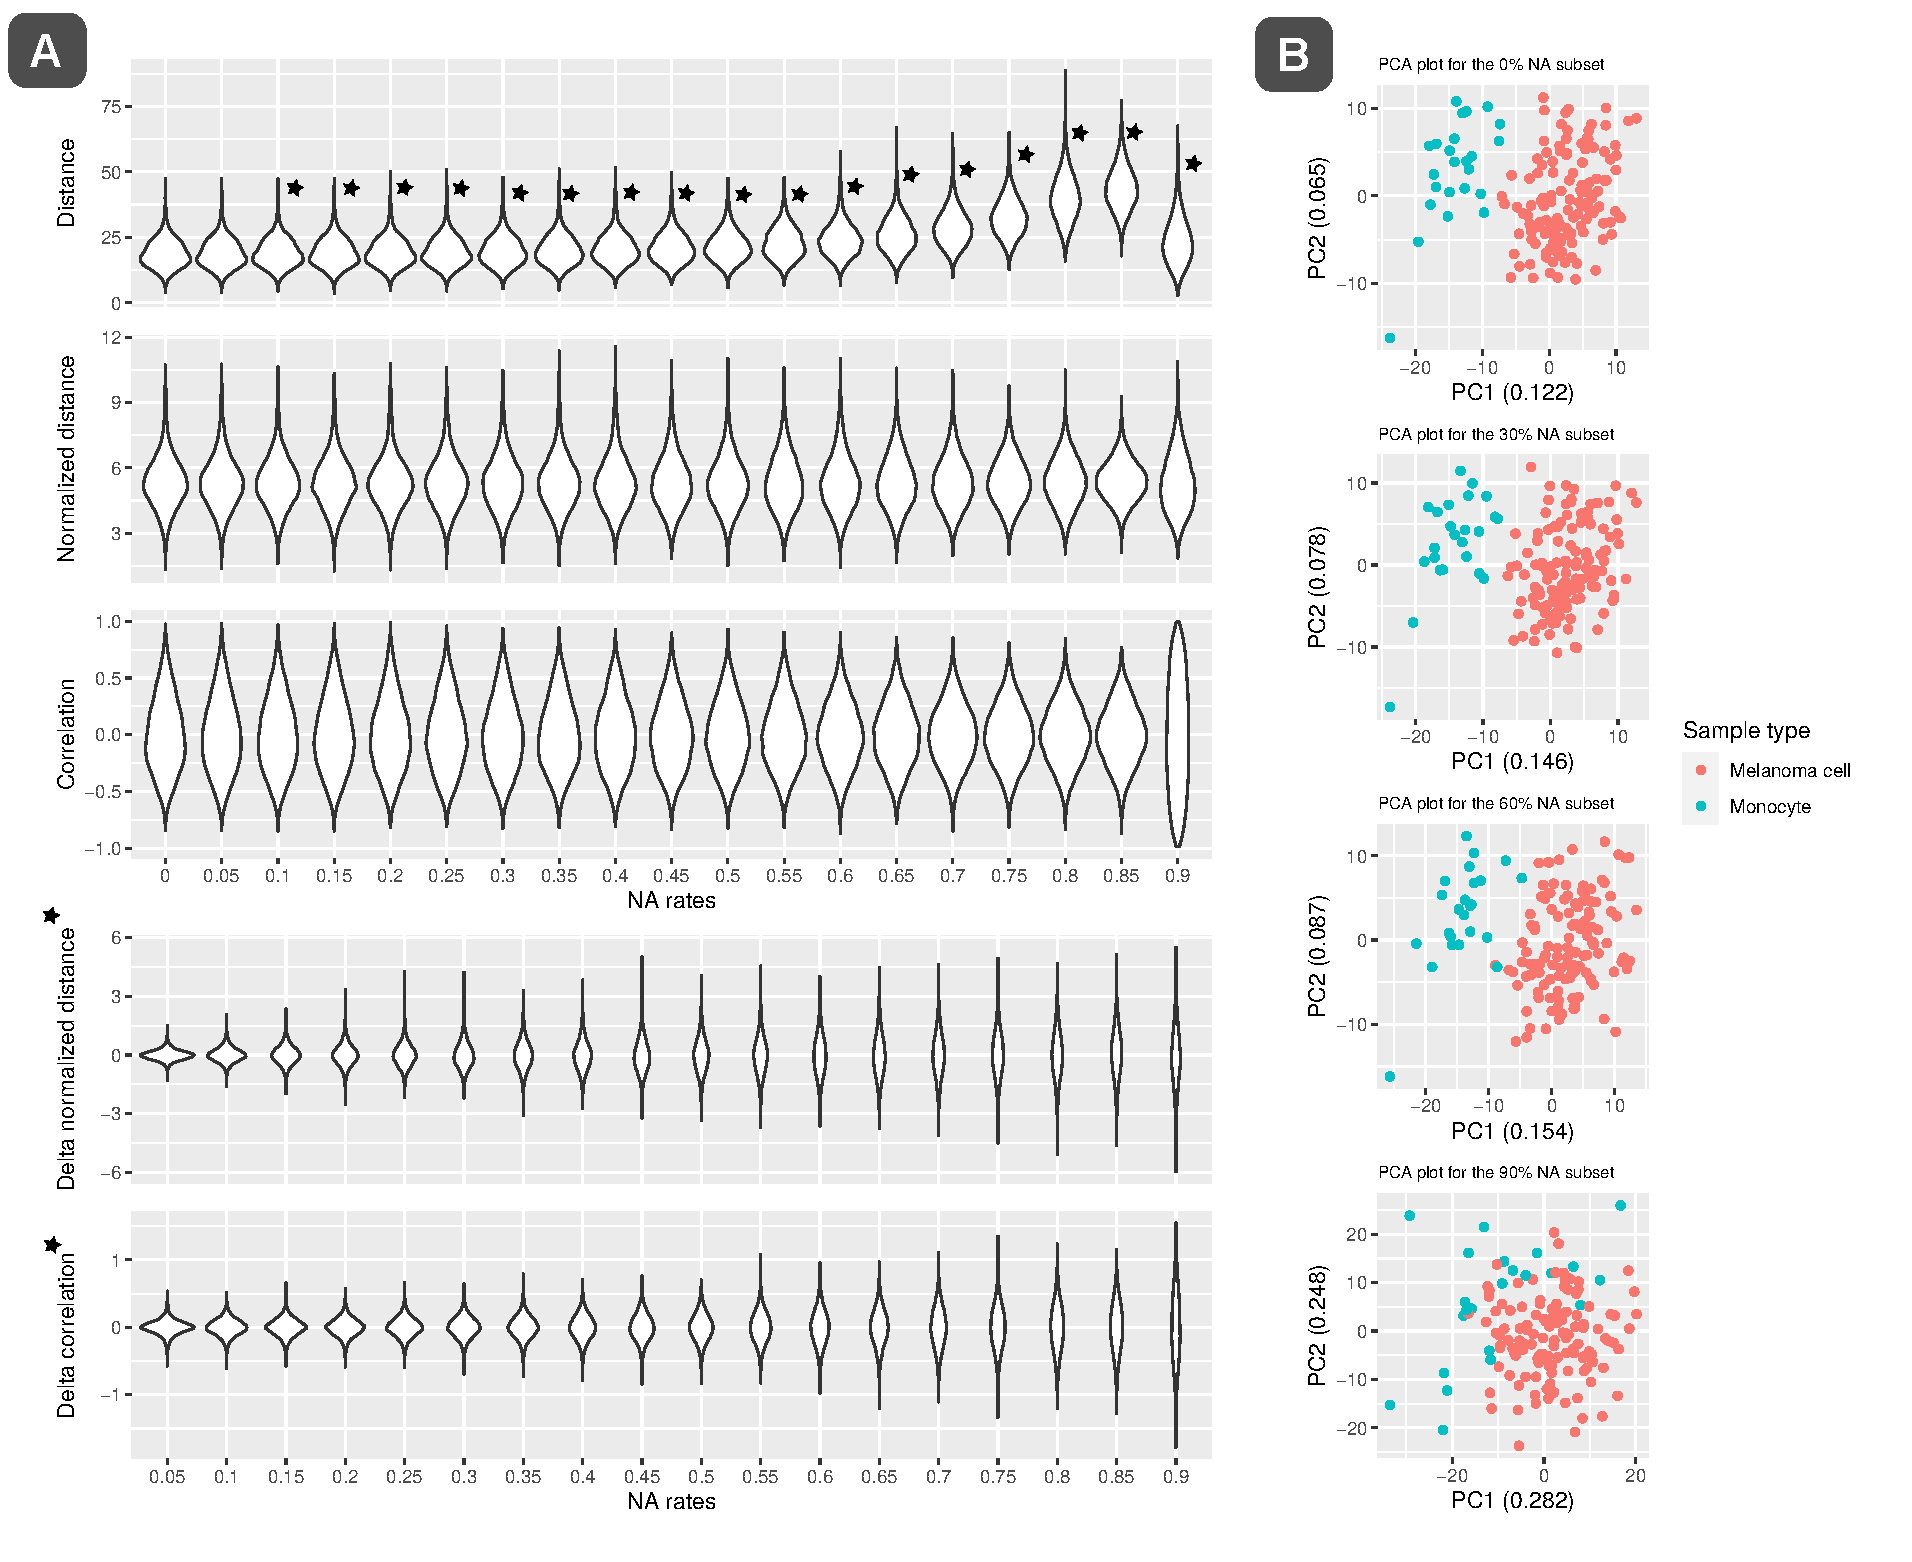
\includegraphics[width = \linewidth]{ppca_combined.pdf}
    \caption{\small (A) Five graphs representing each metric for each missing value rate in the data set. \scriptsize The metrics were computed on the PCA made with ppca from pcaMethods. Be aware that the 3 first graphs start with the 0\% missing value data set but the two last graphs start with 5\% of missing values. Asterisks into graph indicate the pvalue of the linear model test between the result and the reference (first group in the graph) . When asterisks are outside a graph they indicate that the total pvalue is inferior to 0.05
    \small (B) Four PCA plot for 0\%, 30\%, 60\% and 90\% missing value rate. \scriptsize Numbers between parentheses on axis title stand for the proportion of variability that is explained by the PC. Blue points represent Monocyte cells, red points represent Melanoma cells.}
    \label{corr_dist_ppca}
\end{figure*}

To see the changes within the pattern, the same method as for NIPALS was used, the difference between the normalised distance from the PCA obtained with the 0\% missing value data set and the normalised distance from the PCA of each of the other percentage of NA was computed. Same was done using the correlation. Both delta normalised distance and delta correlation show an increase (Levene Test : pvalue <2e-16) in the values of the difference (positively or negatively). This indicates that even if the overall pattern of the cells is similar for all NA rates, the arrangement within the pattern seems to change. This change become bigger as the missing value rate increases. This means that there is an effect of the insertion of missing values, but this effect does not affect the overall pattern of each PCA.

A closer look to some PCA plots (Fig. \ref{corr_dist_ppca} B), shows graphically that the clusters seem to overlap more deeply.


Globally, despite the disparity in term of variation of PC scale (decrease for NIPALS and increase for PPCA), the normalised distance and correlation results show same pattern for NIPALS or PPCA. Both pca methods appear to have a change in the cells arrangement inside patterns when the NA rate increase.  The change in term of correlation and normalised distance difference seems to follow a linear relationship with the missing value rate.  


\subsection{Impact of imputation and missing values on a downstream analysis}

Downstream analysis are often based on PCA results. Therefore comparing the results of downstream analysis can give an idea of the quality of the PCA. Here, the accuracy of the clustering algorithm kmeans on different missing value rates is compared \citep{Rlang}. These results can reflect the amplitude of the separation of the two groups of cells in the PCs dimension.(cf.\ref{accuracy_plot}) 

\begin{figure*}[!ht]
    \centering
    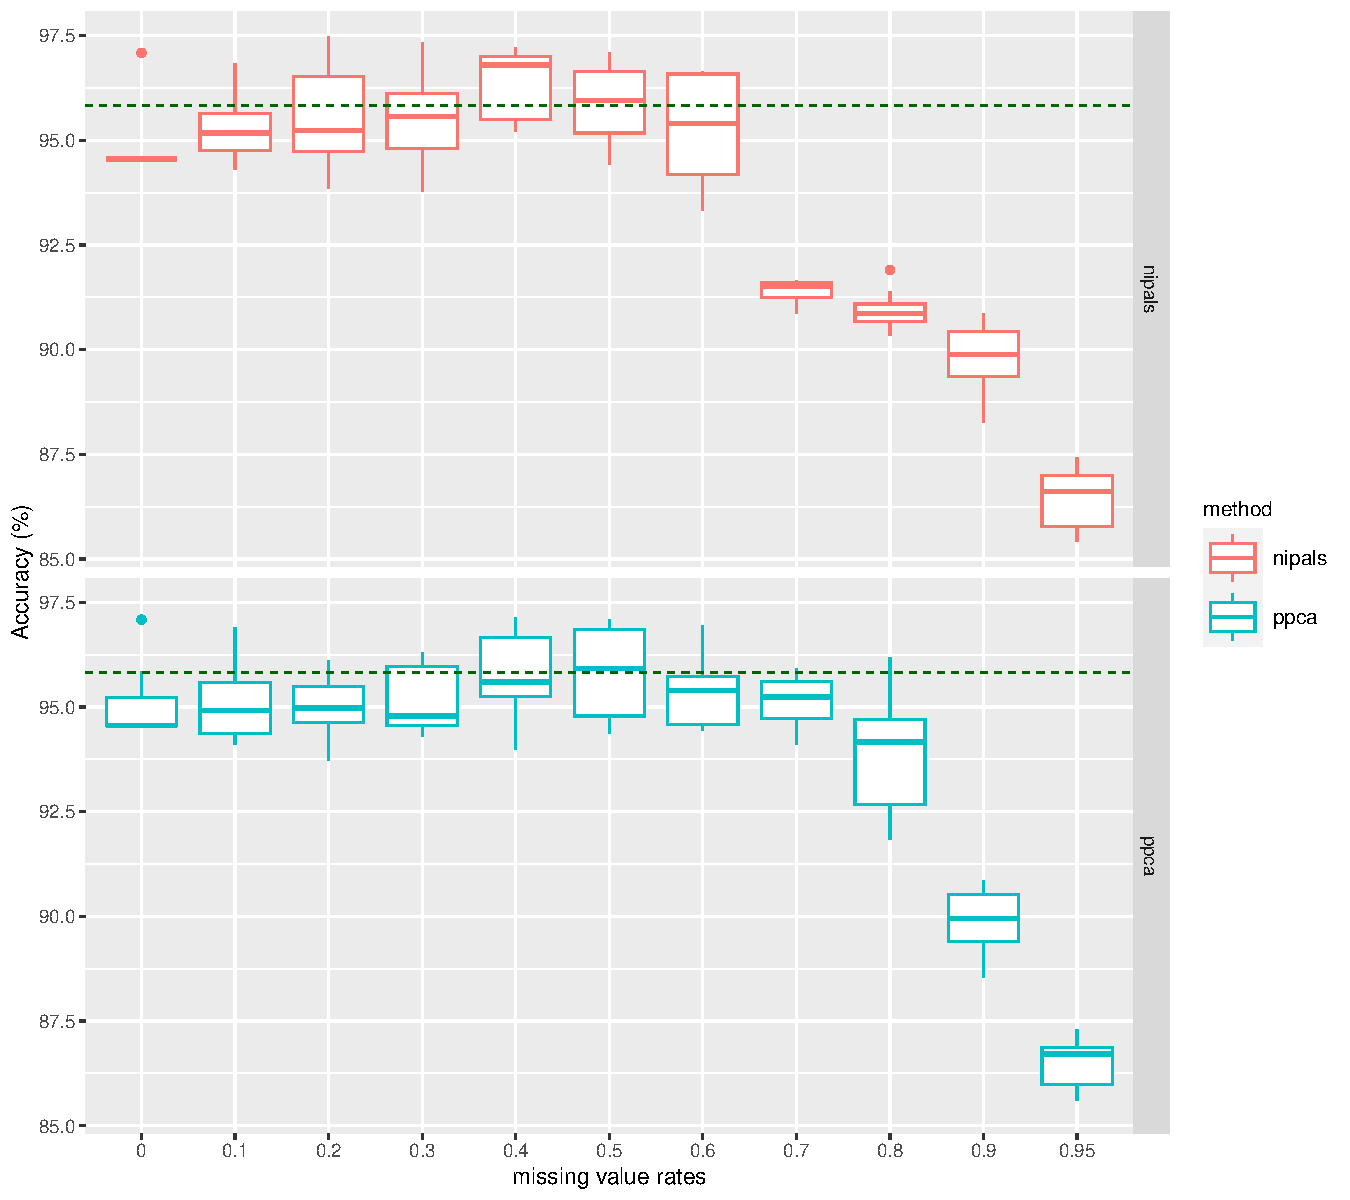
\includegraphics[width = \linewidth]{replication_3_no_random_acc.pdf}
    \caption{\small Graph of the accuracy in percents in function of the missing value rate in the data set, red is for NIPALS and blue for PPCA. \scriptsize Each missing rate value contains 10 accuracy values, corresponding to the replicates. The dashed green line correspond to the mean of the accuracy obtained with the kmeans clustering on the svd PCA with imputed data set (mean = 95,82\%). The method to generate missing values change between the 0.6 and 0.7 missing values (from non-random generation to random). Be aware that the scale change for the last missing value rate (from 0.9 to 0.95).}
    \label{accuracy_plot}
\end{figure*}

First, both algorithms (NIPALS and PPCA \citep{pcaMethods}) seem to follow the same pattern of accuracy in function of missing value rate. This shows that the PCAs obtained with both algorithms are quite similar. But for 70\% and 80\% of missing values, the results are drastically different this could be explained by the fact that PPCA use a imputation step while NIPALS do not consider the NAs.

Surprisingly, there are some outliers even for the 0\% missing value data set, meaning that even with same data, the application dimension reduction and kmeans produce different results. This heterogeneity is highlighted through the use of replicates (n = 10). The key result of this experiment, is that there is an increase of the accuracy as the imputed data get subtracted. This could mean that the imputation hides a part of the biological information contained in the original data. As expected, when the initial values get subtracted (>65\% NAs), the accuracy drops (particularly for NIPALS). This should be due to the fact that the removal of these values cause a lost of real information. Compare to the results obtained with the imputation followed by a svd PCA and a kmeans clustering (dashed green line on Fig. \ref{accuracy_plot}), the accuracy appear to be equivalent for NIPALS and PPCA for missing value rate up to 60\% . This mean that in this case the results obtained with NIPALS and PPCA are reliable. 



\subsection{Time performance of each algorithm}

\begin{figure*}[!ht]
    \centering
    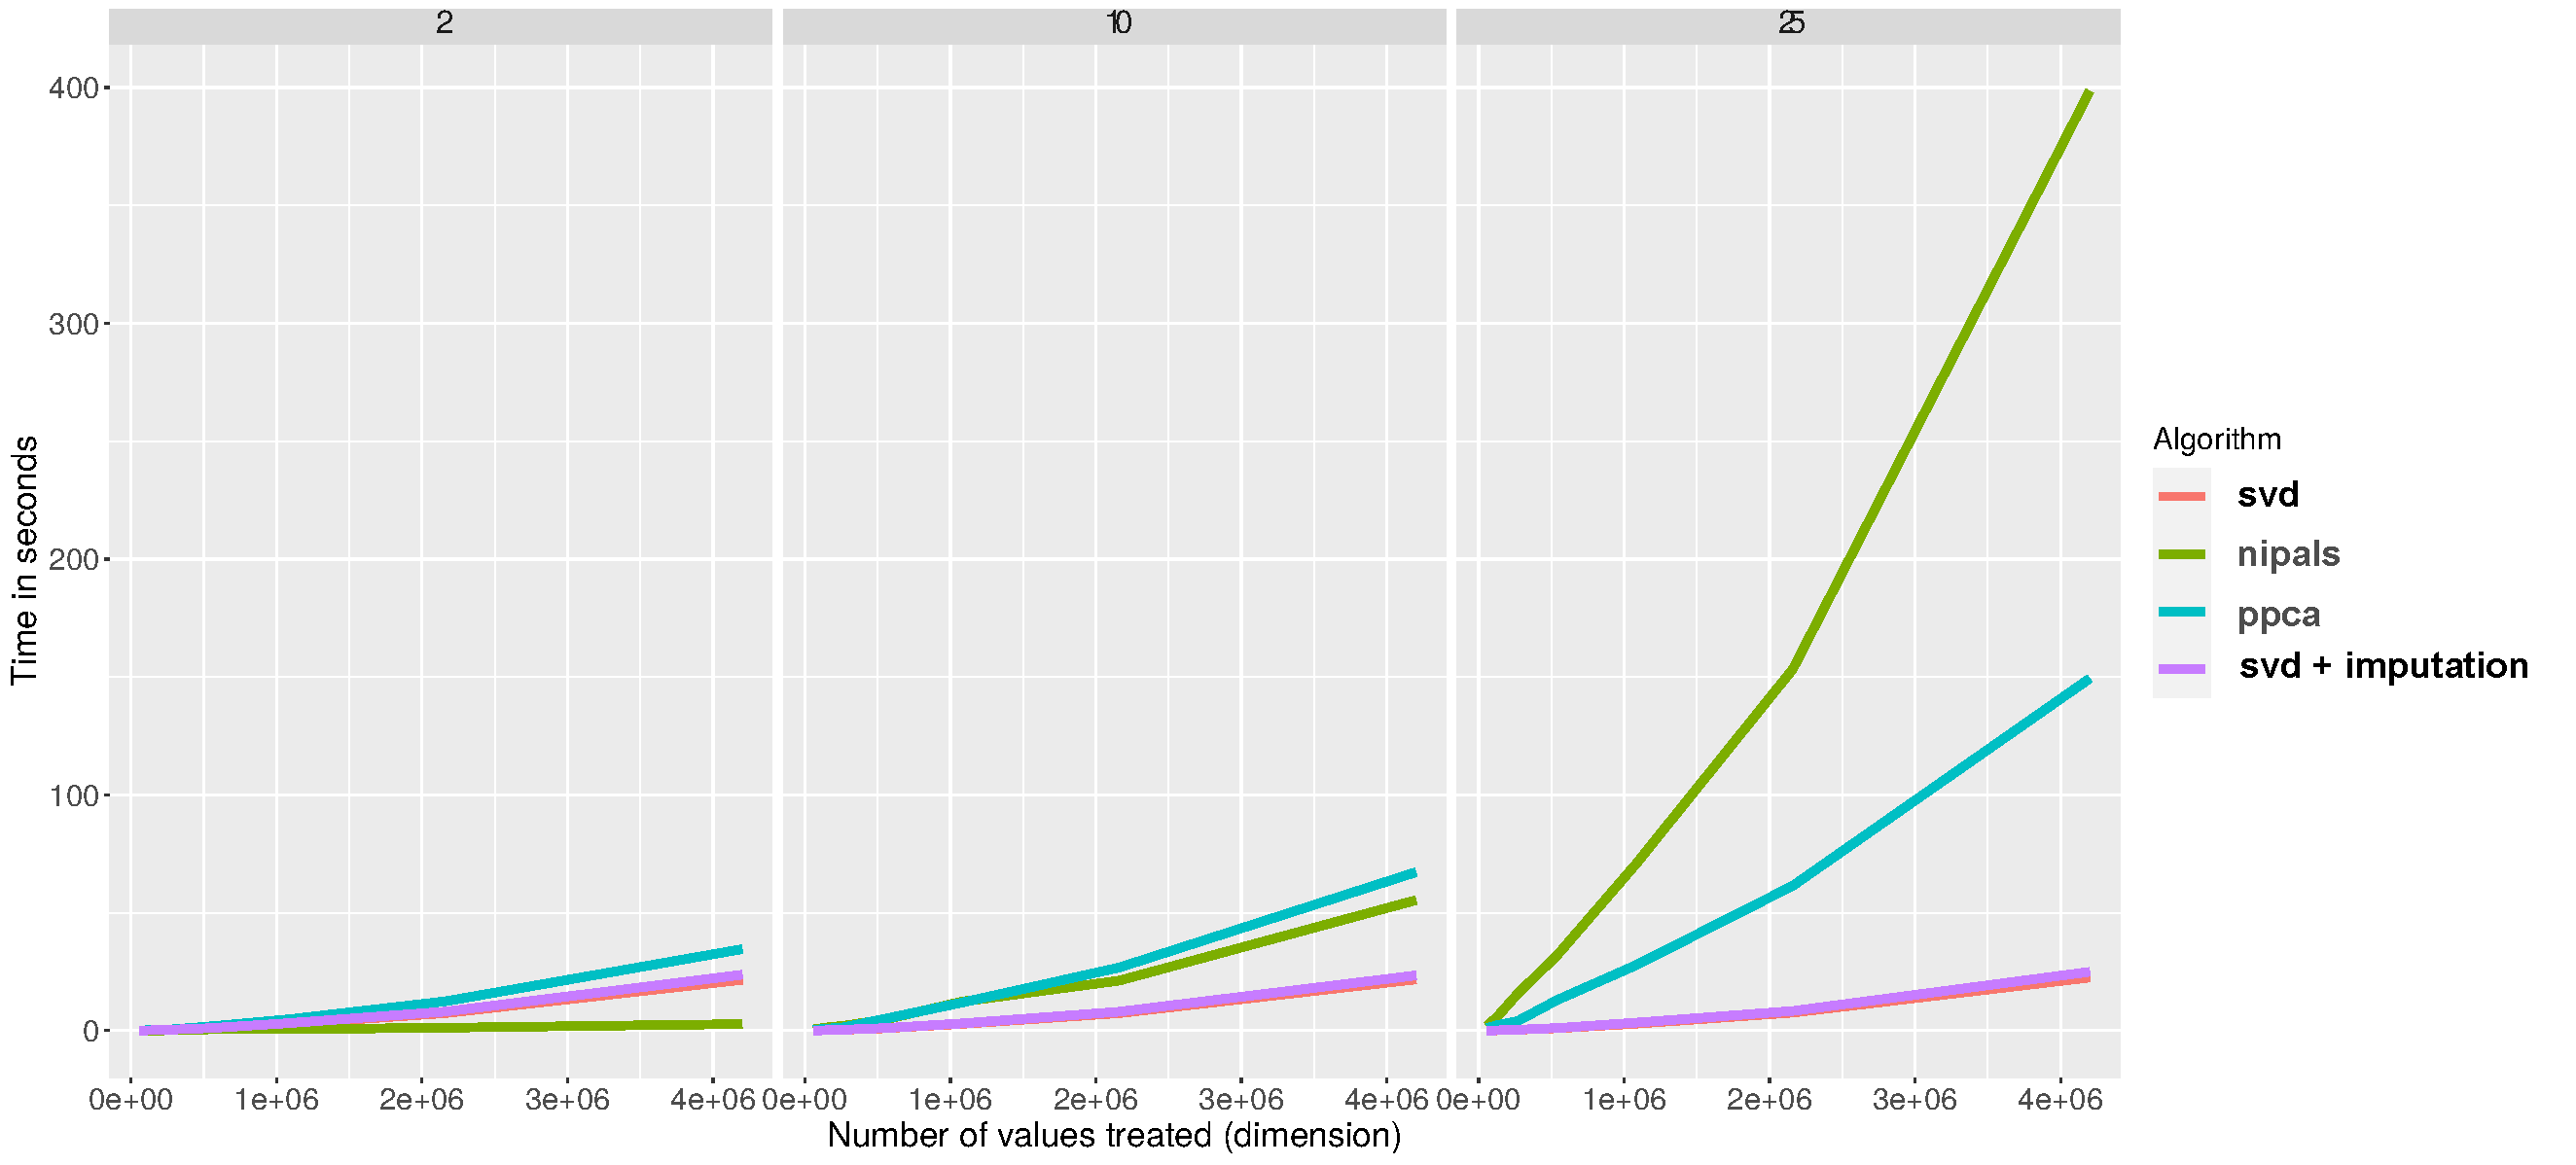
\includegraphics[width =  \linewidth]{bench_cropped.pdf}
    \caption{\small Graphs of the time (in seconds) taken by each algorithm to compute PCA. The x axis represents the data set dimension used. Each graph shows the results for a specific number of PCs. \scriptsize Time was calculated with 60000, 135000, 270000,  540000, 1080000, 2160000, 4200000 values. Be aware that the svd and svd + imputation are partly overlapping (red and purple).
    }
    \label{bench_plot}
\end{figure*}

To have an idea on the time efficiency of the different algorithms, a benchmark of each algorithm was made. Benchmark was realise with different subsets dimension and for a different number of PCs to compute.

Several observations can be drawn from the benchmark performed.  First, the time taken by svd remains stable according to the number of PCs calculated. This is due to the fact that svd computes in all cases all PCs and then subsets the number of PCs asked. Second, the execution time of NIPALS and PPCA is strongly impacted by the number of PCs requested. This is especially true for NIPALS. With 2 PCs calculated, NIPALS is the best, even surpassing svd. But with the increase in PCs, the time required by NIPALS increases rapidly, so that PPCA becomes faster than NIPALS (25 PCs). These results can be explained by the fact that NIPALS compute a PC and iterate on it, then repeating the same method for each PC. As for PPCA, the algorithm compute each PCs asked and then iterate on all the PCs on the same time. 
Third, the time taken by the imputation itself is not significant. Indeed, for the 3 graphs proposed in figure \ref{bench_plot}, the difference between the calculation of svd + imputation is not strongly different from the calculation of svd alone.It is also important to note that even in the worst case (with 25 PCs and >4e+6 dimension) the time required by NIPALS remains reasonable since it executes in less than 7 minutes.


\section{Discussion}

The first results obtained by measuring the distances and the correlations, show that the variation produced by the insertion of missing values increases in a linear way. Thanks to the PCA plots, it is visible that the insertion of missing value increases the overlap between the two groups of cells. All this indicates that adding missing values deteriorates the quality of PCAs. But this effect is not particularly strong under 70\% - 80\% of missing values. The PCAs seem to stay reliable under these values.

The second analysis shows the effect of using an alternative PCA under real analysis conditions. This analysis shows that NIPALS and PPCA remain reliable when the data are not imputed. Nevertheless, PPCA use an imputation step in his algorithm. Thus NIPALS would be the good alternative to PCA involving imputation. This would remove all the negative points related to the imputation. 

However, it is important to keep in mind that although this alternative method appear to perform well, it does not mean that it is perfect. Indeed, the major flaw of PCA without imputation is that missing values are simply ignored. It would be wise to take into account these missing values as being possibly biologically significant. Models attempting to carry out this heavy task have already been developed in other fields, in single cell RNA sequencing\citep{risso_general_2018} and in proteomic\citep{goeminne_msqrob_2020, obrien_effects_2018}. It would therefore be interesting to develop such models within the framework of single cell proteomic.
Other methods, such as bpca \citep{oba2003bayesian} and MissMDA \citep{missMDA} that allow the use of PCA to overcome the problem of missing values should also be evaluated within the SCP frame.

To enhance the comparison of the time performance of each algorithm, it could be an good idea to test them with different parameters, such as number of iterations or the threshold value used.  

\section{Conclusion} 
In view of the results obtained in this report, performing PCAs with NIPALS and PPCA on non-imputed data seems to be reliable for data sets with up to 70\% - 80\% of NAs. The results obtained with these methods are not different from those obtained with svd + imputation. 
In the context of the SCP, as PPCA use an hidden imputation step, it would be preferable to use NIPALS without imputation. This would remove all the problems brought by the imputation.

But it's also important to keep in mind the practicality of using these methods. In fact, NIPALS appear to not scale very well with the increase of computed PCs asked. Therefore, for downstream analysis, where the number of PCs should be high, the time taken by NIPALS should be consider.

%\printbibliography

\bibliography{references}

\end{document}